


\section{Factores que afectan la velocidad de reacción}

Existen diversos parámetros que pueden afectar la velocidad con la que ocurre una reacción enzimática.

\subsection{Aspectos fisico-químicos}

Puesto que las enzimas son al final del día proteínas, debemos recordar las variables que pueden desnaturalizar una proteína, pues también afectan a las enzimas. Las principales variables son la temperatura y el pH. Hay que recordar también que estas variables cambian de enzima a enzima. Por ejemplo, mientras que cierta enzimas si pueden funcionar a temperaturas altas, existen otras que no, y viceversa. Otro punto a tomar en cuenta es que no se trata de estados de ``encendido y apagado''. Por ejemplo, una enzima que funciona a temperatura ambiente no perderá actividad de manera abrupta cuando se suba la temperatura, sino que irá perdiendo poco a poco la actividad conforme se va subiendo la temperatura.

Por todo esto, cada vez que exista una enzima que sea de nuestro interés es necesario conocer este tipo de parámetros, para poder mantener, por ejemplo, nuestro biorreactor, a las condiciones óptimas de funcionamiento de nuestra enzima.

\subsection{Inhibidores}

Existen sustancias que pueden reducir la velocidad de reacción al ``bloquear'' el funcionamiento correcto de la enzima. 

\subsection{Tipos de inhibición enzimática}

Estos se pueden clasificar de la siguiente manera:

\begin{itemize}
    \item Competitivos: Se unen al sitio catalítico y acaparan el lugar donde el sustrato entraría. Una forma de compensar la reducción de velocidad por estos inhibidores es añadir sustrato, para que ``le ganen el lugar'' al inhibidor.
    \item No competitivos: Estos se unen a otras partes de la enzima que desactivan el sitio catalítico, por lo que aunque el sustrato si se puede unir, la reacción no se lleva a cabo. Añadir sustrato no funciona aquí.
    \item 
\end{itemize}

\begin{figure}[H]
    \centering
    \begin{subfigure}{0.485\textwidth}
        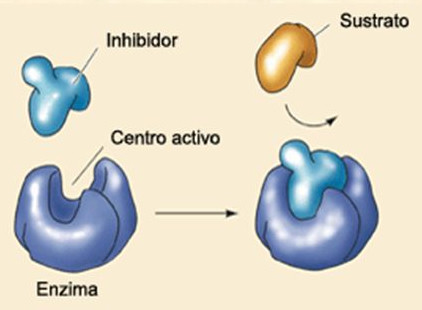
\includegraphics[width=\linewidth]{images/fig:inhibicion_competitiva}
        \caption{\textbf{Competitivo:} Aquí se muestra como el inhibidor toma lugar en el sitio activo, bloqueando la entrada del sustrato}
    \end{subfigure}
    \hspace*{\fill}
    \begin{subfigure}{0.485\textwidth}
        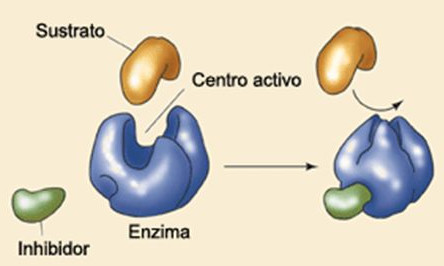
\includegraphics[width=\linewidth]{images/fig:inhibicion_no_competitiva}
        \caption{\textbf{No competitivo:} A diferencia del anterior, el sustrato si se une, pero no se lleva a cabo la reacción porque el inhibidor "bloquea" el trabajo del sitio activo.}
    \end{subfigure}
    
    \rule{\linewidth}{0.2pt}
    \caption[Tipos de inhibición enzimática]{Tipos de inhibición enzimática}
    \label{fig:tipos_de_inhibición_enzimática_ilustrado}
\end{figure}

\marginpar{
\begin{minipage}{\marginparwidth}
    \begin{figure}[H]
        \centering
        \begin{subfigure}{\linewidth}
    \centering
    \resizebox{\linewidth}{!}{
    \begin{tikzpicture}
        \draw[-Stealth, line width=0.5pt] (-5,0) -- (10,0) node[below=5pt, font=\Huge] {$\frac{1}{V}$};
        \draw[-Stealth, line width=0.5pt] ( 0,0) -- (0,10) node[xshift=-2.5em, font=\Huge] {$\frac{1}{[S]}$};
        \draw[red,  line width=0.5pt] (-2,0) -- (3,9);
        \draw[blue, line width=0.5pt] (-4,0) -- (5,8);
    \end{tikzpicture}
    }
    \rule{\linewidth}{0.2pt}
    \caption{Inhibición competitiva}
\end{subfigure}

\vspace*{10pt}

\begin{subfigure}{\linewidth}
    \centering
    \resizebox{\linewidth}{!}{
    \begin{tikzpicture}
        \draw[-Stealth, line width=0.5pt] (-5,0) -- (10,0) node[below=5pt, font=\Huge, midway] {$\frac{1}{V}$};
        \draw[-Stealth, line width=0.5pt] ( 0,0) -- (0,10) node[xshift=-2.5em, font=\Huge] {$\frac{1}{[S]}$};
        \draw[red,  line width=0.5pt] (-3.5,0) -- (3.5,8.5);
        \draw[blue, line width=0.5pt] (-1.5,0) -- (5.5,8.5);
    \end{tikzpicture}
    }
    \rule{\linewidth}{0.2pt}
    \caption{Inhibición incompetitiva}
\end{subfigure}

\vspace*{10pt}

\begin{subfigure}{\linewidth}
    \centering
    \resizebox{\linewidth}{!}{
    \begin{tikzpicture}
        \draw[-Stealth, line width=0.5pt] (-5,0) -- (10,0) node[below=5pt, font=\Huge, midway] {$\frac{1}{V}$};
        \draw[-Stealth, line width=0.5pt] ( 0,0) -- (0,10) node[xshift=-2.5em, font=\Huge] {$\frac{1}{[S]}$};
        \draw[red,  line width=0.5pt] (-2,0) -- (3,9);
        \draw[blue, line width=0.5pt] (-2,0) -- (5,8);
    \end{tikzpicture}
    }
    \rule{\linewidth}{0.2pt}
    \caption{Inhibición no competitiva}
\end{subfigure}
        \rule{\linewidth}{0.2pt}
        \caption[Tipos de inhibición enzimática graficados]{Diferencia entre los tipos de inhibición enzimática. Las gráficas representan los efectos de diferentes tipos de inhibidores en la linearización por método de Lieneawever-Burk}
        \label{fig:tipos_de_inhibicion_enzimatica}
    \end{figure}
\end{minipage}
}

\subsubsection{Competitiva}



\subsubsection{No competitiva}



\subsubsection{Acompetitiva}



\subsubsection{Mixta}


